%%%%%%%%%%%%%%%%%%% Especificación:
\begin{frame}[fragile]{Vector Clocks in Action:}{Immediate Precessors}
    \justifying
    \textbf{El problema del seguimiento del predecesor inmediato (Immediate predecessor tracking IPT)} 
    Consiste en asociar a cada evento relevante el conjunto de eventos relevantes que son sus predecesores inmediatos.

    Además, esto se ha hecho sobre la marcha y sin añadir mensajes de control.
    
    La determinación de los predecesores inmediatos consiste en calcular la reducción transitiva (o diagrama de Hasse) del orden parcial $\widehat{R}=(R,\xrightarrow[]{re})$. 

    \justifying
    \begin{figure}
        \begin{subfigure}[b]{\textwidth}
            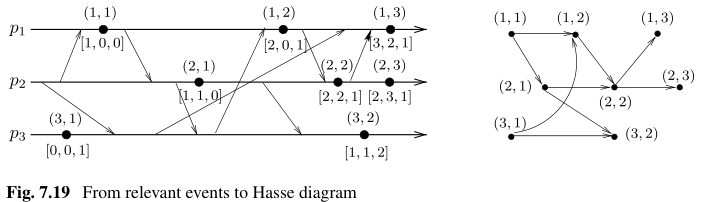
\includegraphics[scale=0.7]{Imagenes/eventosRelevantes03.png}
            \label{fig:ejemplo2}
        \end{subfigure}
    \end{figure}

\end{frame}